\section{Auswertung}
	\label{sec:Auswertung}

	\subsection{Bestimmung des Dunkelstroms}
		\label{sub:bestimmung_des_dunkelstroms}
		
		Um die Messwerte mit der Theorie vergleichen zu k"onnen muss zuerst der Dunkelstrom $I_\mathrm{du}$ gemessen werden.

		Dazu wurde unter Versuchsbedingungen, jedoch mit ausgeschaltetem Laser, eine Messung durchgef"uhrt.

		F"ur den Dunkelstrom ergab sich:

		\begin{equation}
			I_\mathrm{du} = \SI{0.13}{\nano \ampere}
		\end{equation}

		Die Aufgetragenenen Messwerte in den Tabellen sind noch nicht um diesen Wert reduziert.

	\subsection{Bestimmung der Spaltbreite eines festen Einfachspalts}
		\label{sub:bestimmung_der_spaltbreite_eines_festen_einfachspalts}
		
		Im folgenden wird die Spaltbreite eines Einfachspalts auf zwei verschiedene Weisen gemessen. Einmal mithilfe des Beugungsmusters und einmal mit Hilfe eines Mikroskops.

		\subsubsection{Bestimmung mit Hilfe des Beugungsmusters}
			\label{sub:Bestimmung_mit_Hilfe_des_Beugungsmusters}

			Wie die Spaltbreite bestimmt wird, wird bereits in \ref{sec:messung} erl"autert. Die bereinigten Messwerte finden sich in Tabelle \ref{tabelle_1} wieder.

			Die gemessene Intensit"at wurde in Grafik \ref{graf_1} gegen die Detektorposition aufgetragen und eine Theoriekurve nach Gleichung \ref{prop_einzelspalt} eingef"ugt um die Kurven vergleichen zu k"onnen.

			Zur Anpassung wurde PyPlot benutzt.

			Es ergibt sich mithilfe der Formel:

			\begin{equation}
				f(x) = a^2 b^2 \left(\frac{\lambda}{\pi b sin(\frac{x-x_\mathrm{0}}{d})}\right)^2 sin^2 \left( \frac{\pi b sin(\frac{x-x_\mathrm{0}}{d})}{\lambda} \right)
			\end{equation}

			f"ur die Werte ergaben sich:

			\begin{table}[h]
\begin{center}
\begin{tabular}{c|c|c||c|c|c||c|c|c}
Ub[V] & Ud[V] & D[1/4 in] & Ub[V] & Ud[V] & D[1/4 in] & Ub[V] & Ud[V] & D[1/4 in] \\
\hline
200 & -7,1 & 4 & 250 & -9,3 & 4 & 300 & -11,9 & 4 \\
200 & -3,9 & 3 & 250 & -5,2 & 3 & 300 & -7,1 & 3 \\
200 & -0,1 & 2 & 250 & -0,4 & 2 & 300 & -1,2 & 2 \\
200 & 3,4 & 1 & 250 & 4 & 1 & 300 & 4,3 & 1 \\
200 & 6,9 & 0 & 250 & 8,4 & 0 & 300 & 9,5 & 0 \\
200 & 10,5 & -1 & 250 & 12,6 & -1 & 300 & 14,8 & -1 \\
200 & 13,7 & -2 & 250 & 17,3 & -2 & 300 & 20,4 & -2 \\
200 & 17,4 & -3 & 250 & 21,4 & -3 & 300 & 25,3 & -3 \\
200 & 20,7 & -4 & 250 & 25,4 & -4 & 300 & 30,0 & -4 \\
\end{tabular}
\caption{Messwerte zu Aufgabe a bei verschiedenen Beschleunigungsspannungen}
\label{tabelle_1}
\end{center}
\end{table}
			\input


			blablabla auswertung

		\subsubsection{Bestimmung mit Hilfe des Mikroskops}
			\label{sub:Bestimmung_mit_Hilfe_des_mikroskops}

			Das Ausmessen mithilfe des Mikroskops wurde bereits in \ref{sec:messung_mikro} erkl"art.
			Es wurde auf das Objektmikrometer fokussiert. Nun wurde der Spalt unter das Objektiv gelegt und mithilfe eines verschiebbaren Teilstrichs die Spaltkanten "uberdeckt. Diese Fixierung wurde dann auf die Mikrometerskala des Objektmikrometers gelegt und ausgemessen.
			Aufgrund von Unsch"arfen wurde ein Fehler von $\sigma_0 = \SI{10}{\micro \meter}$ angenommen.

			Es ergab sich f"ur die Spaltbreite b:

			\begin{equation}
				b = \SI{70}{\micro \meter}
			\end{equation}

			Damit ergibt sich f"ur die gemessene Spaltbreite $b_\mathrm{mikro} = \SI{70 (10)}{\micro \meter}$.
			Es besteht ein gro"ser Unterschied zwischen der gemessenen und der angegebenen Spaltbreite von $b = \SI{80}{\micro \meter}$.
			Auf Fehlerquellen wird in der Diskussion eingegangen.

			\newpage

	\subsection{Bestimmung der Spaltbreite eines variablen Einfachspalts} 
		\label{sub:bestimmung_der_spaltbreite_eines_variablen_einfachspalts}
		
		Nun sollte die Breite $b$ eines variablen Einfachspalts gemessen werden. Das Messverfahren ist dasselbe wie zuvor.

		Die dazugeh"origen Intensit"atswerte abh"angig von der Detektorposition finden sich in Tabelle \ref{tabelle_2}. Weiter wurde eine Theoriekurve in die Grafik \ref{graph1} einge"ugt, sodass ein Vergleich zwischen Theorie und Experiment m"oglich ist. Daf"ur wurde Gnuplot verwendet.

		Es ergab sich:

		\begin{equation}
			b = \SI{7.46 (170)}{\micro \meter}
		\end{equation}

		\begin{table}[h]	
\centering
\begin{tabular}{|l l||l l||l l|} \hline
	x[mm] & I[nA] & x[mm] & I[nA] & x[mm] & I[nA]\\
	\hline
	0	&	2.5   &  17	&	15  & 34	&	4.8\\
	1	&	2.1   &  18	&	13  & 35	&	3\\
	2	&	2.1   &  19	&	12.5& 36	&	1.85\\
	3	&	2.5   &  20	&	23.5& 37	&	1.55\\
	4	&	2.9   &  21	&	50  & 38	&	2.1 \\
	5	&	2.85  &  22	&	98  & 39	&	2.85\\
	6	&	2.5   &  23	&	135 & 40	&	3\\
	7	&	2.75  &  24	&	165 & 41	&	2.8\\
	8	&	4     &  25	&	155 & 42	&	1.95\\
	9	&	6.2   &  26	&	125 & 43	&	1\\
	10	&	8     &  27	&	92  & 44	&	0.6\\
	11	&	7.9   &  28	&	50  & 45	&	0.51\\
	12	&	6     &  29	&	25.5& 46	&	0.72\\
	13	&	4     &  30	&	11  & 47	&	0.86\\
	14	&	4.8   &  31	&	7.2 & 48	&	0.86\\
	15	&	8.5   &  32	&	6.4 & 49	&	0.68\\
	16	&	13    &  33	&	6   & 50	&	0.45\\
	\hline
\end{tabular}
\caption{Intensit"at des festen Einfachspalts abgh"angig von der Detektorstellung x}
\label{tabelle_2}
\end{table}



		\begin{figure}[h]
			\centering
			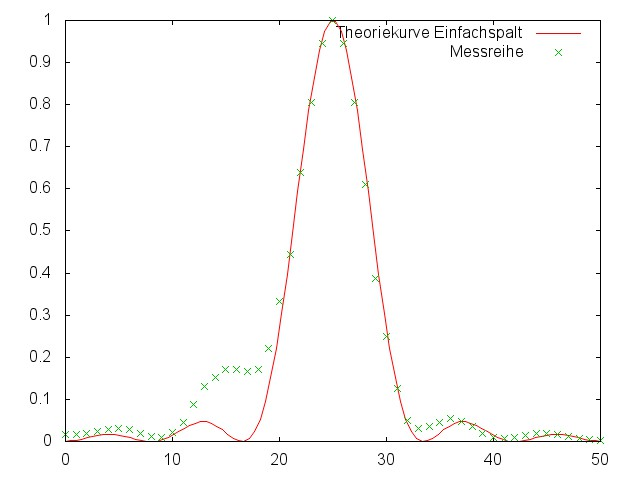
\includegraphics[width = 14cm]{graph1.jpg}
			\caption{Graphische Darstellung der des festen Einfachspalt}
			\label{graph1}
		\end{figure}